% Chapter Template

\chapter{On-Board Integration} % Main chapter title

\label{Chapter4} % Change X to a consecutive number; for referencing this chapter elsewhere, use \ref{ChapterX}

%----------------------------------------------------------------------------------------
%	SECTION 1
%----------------------------------------------------------------------------------------

\section{Tools Introduction}

\subsection{Hybrid Memory Cube and Micron AC-510}


\textsl{Hybrid Memory Cube} (HMC) is a high-performance \textsl{RAM} interface for stacked \textsl{DRAM} memory. Combining \textsc{through-silicon vias} and \textsl{microbumps}\footnote{ (WIKIPEDIA) } to connect multiple layers of memory cells on top of each others, it offers very high throughput parallel serial bus' for random I/O's. In the scope of this project, it is an ideal candidate as to where to store all the references for the  FM-Index string matching algorithm as a parallel solution would indeed query for information potentially dispatched all over the memory.


\subsection{Board and Project Architecture}

The board introduced in the previous section is presented in Figure \ref{fig:board_schema}. It actually consists of 6 \textsl{AC-510} boards plugged onto a \textsl{EX-700} carrier board. This enables simultaneous use of several \textsl{AC-510} with one host connected by one bus. \\

In the project architecture for each \textsl{AC-510} board, several pre-defined \textsl{IPs}, provided by the board manufacturer, are used. A diagram representing the whole project hierarchy and coarse interconnections is presented in Figure \ref{fig:block_diag}. The different \textsl{IPs} and blocks have the following utility\footnote{Picodoc} :


\begin{description}
\item [HMC Controller] - This block offers an interface with the \textsl{HMC} internally for the \textsl{FPGA}, but also directly from the host (via PCIe), through the \textsl{FPGA}. Everything that comes and goes to the \textsl{HMC} passes through this block
\item [HMC Stream Controller ] - This blocks mainly has the same purpose that the previous one, except that it enables the communication between the \textsl{Pico-FrameWork} buses and the \textsl{HMC}.
\item [Pico Framework] - This \textsl{IP} provides a memory-mapped bus, the  \textsl{PicoBus}. It is used to initialize the \textsl{AC-510} device as well as configuring and using it via control/status registers and an PCIe bus.
\item [Pico Stream Controller] - This block, as well as the \textsl{HMC Stream Controler}, is used as an interface between a \textrm{256-bit} wide stream bus and an adapted \textrm{128bits} wide bus, used by the internal modules (e.g. \textsl{reds\_top}. This conversion is also necessary for the \textsl{HMC Stream Controller} to communicate  \textsl{PicoBus} data to/from the \textsl{HMC}.
\item [UserWrapper] - This block, as its name states, is used as a wrapper for any user application in the project. It enables a hierarchical architecture, much simpler to read and use, providing only the "stream adapters" \textsl{HMC Stream Contoller} and \textit{Pico Stream Controller}.
\item [Reds\_top \& FM-Index\_top ] - Those blocks are mainly used to keep a good hierarchical design by encapsulating case specific blocs in the global reusable project.
\end{description}


\begin{figure}[H]
    \centering
    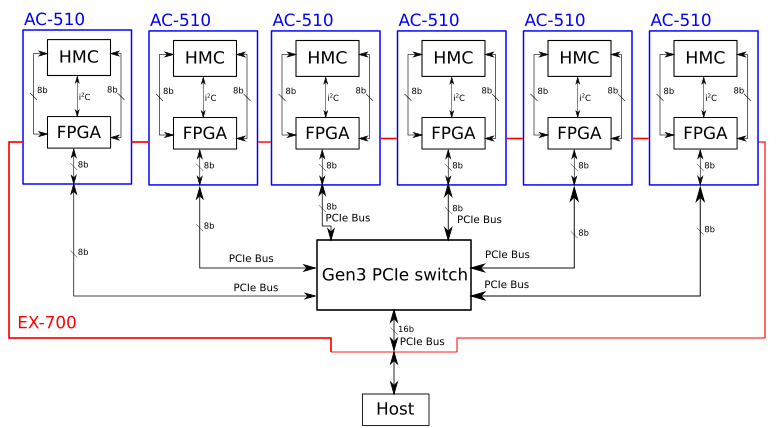
\includegraphics[scale = 0.4]{Figures/pico_board.png}
    \caption{Bloc Diagram of the Board}
    \label{fig:board_schema}
\end{figure}

\begin{minipage}[t]{0.6\textwidth}
\begin{figure}[H]
  \hspace{-15mm}  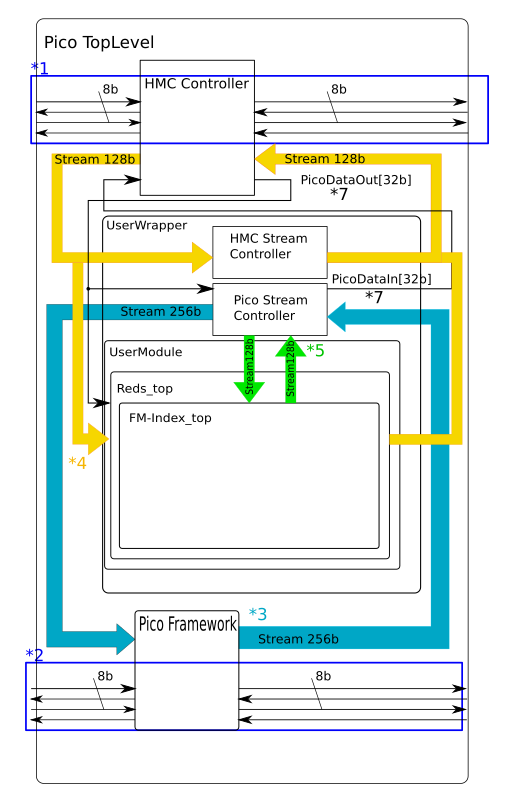
\includegraphics[scale = 0.6]{Figures/block_diagram.png}
    \caption{Bloc Diagram of the whole project}
    \label{fig:block_diag}
\end{figure}
\end{minipage}
\begin{minipage}[t]{0.35\textwidth}
Below are defined the differents references places on the Figures \ref{fig:block_diag} :
\begin{description}
\item [1] PCIe bus interface around the HMC controller, different from the \textrm{128-bit} wide bus used internally
\item [2] 8 parallel PCIe serial bus' for the \textsl{Pico Framework}, directly accessible from the host.
\item [3] Internal \textrm{256-bit} wide bus used to communicate with the lower-level design and the HMC.
\item [4] Internal \textrm{128-bit} wide bus used to communicate with the lower-level entity designed in this project and the \textsl{PicoBus}
\item [5] Internal \textrm{128-bit} wide bus used to communicate between the lower-level design and upper-level entities (e.g. host)
\item [6] \textrm{32-bit} wide direct bus between the \textsl{HMC Controller} and the lower-level entity designed in this project.
\end{description}
\end{minipage}

\section{Integration into the PicoBaseProject}


\subsection{Additional Blocs}



\begin{description}
\item [PCI Interface] - This bloc is the interface between the \textsl{PCI Express Bus} and the FM-Index bloc. It receives short reads and command from a master. In this interface, the FM-Index bloc is a slave, that wait for commands and data to start working. A FIFO is already implemented and this bloc consumes what is put into it. When a result is ready, it is placed in another FIFO that can be accessed by the computer master on the other end.
\item[Pico Bus Interface] - In order to enable addressed registers to configure the \textit{Occ} and \textit{LEN\_BWT} parameters, it seemed necessary to implement an interface to the PicoBus. The particularity of this bus is that it does not share the same clock that the rest of the system. It has indeed its own clock, expected to be much slower that the main one. This requires some level of synchronization in order to ensure the absence of metastable state of the written values. Thus, this bloc is in charge of listening to the address bus of the PicoBus interface in order to detect software originated writes. If one of those transaction is destined to one of the FM-Index internal parameters, it forwards the correct values to the central bloc.
\item [HMC Interface] - Similarly to the first bloc, this one is the interface between the board main memory and the FM-Index bloc. Only accessed through the \textsl{Memory Query} bloc, it is used to query data, may it be checkpoints entries, BWT entries of Sampled Suffix array elements. All transactions are 128-bit wide and the interpretation of the received data in the \textsl{Memory Query} bloc.
\item [Memory Query] - This bloc is used by the FM-Index to issue all the different queries it might need along the string matching process, which means it implements all 3 "functions" needed by the FM-Index : $Occ$, $Count$ (thus $LF$) and $Walk-Left$ (with the sampled suffix array). Those queries can be about "checkpoints", BWT symbol or sampled suffix array entries and the type of said requests is specified by the \textrm{req\_type} signal. This bloc is then responsible for interpreting the received data and transmitting it in the appropriate form to the FM-Index bloc. Note that in the actual implementation, this bloc is part og the HMC Interface bloc.
\end{description}

\subsection{Reds\_Top}
\begin{figure}[H]
    \centering
    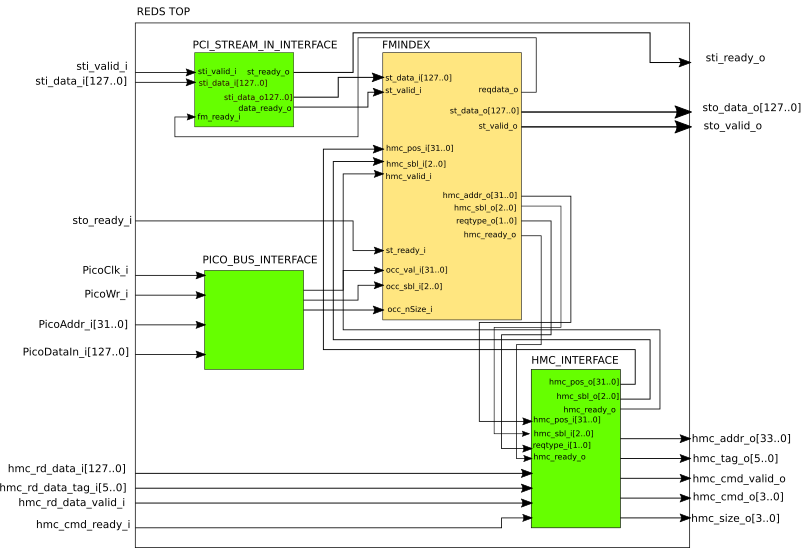
\includegraphics[scale = 0.55]{Figures/REDS_TOP_DIAG.png}
    \caption{reds\_top Bloc Diagram}
    \label{fig:reds_top_diag}
\end{figure}

\subsection{PCI Interface}
TODO
SCHEMA BLOC, FSM

\subsection{PicoBus Interface}
TODO
\subsection{HMC Interface}

\begin{figure}[H]
    \centering
    \hspace*{-20mm}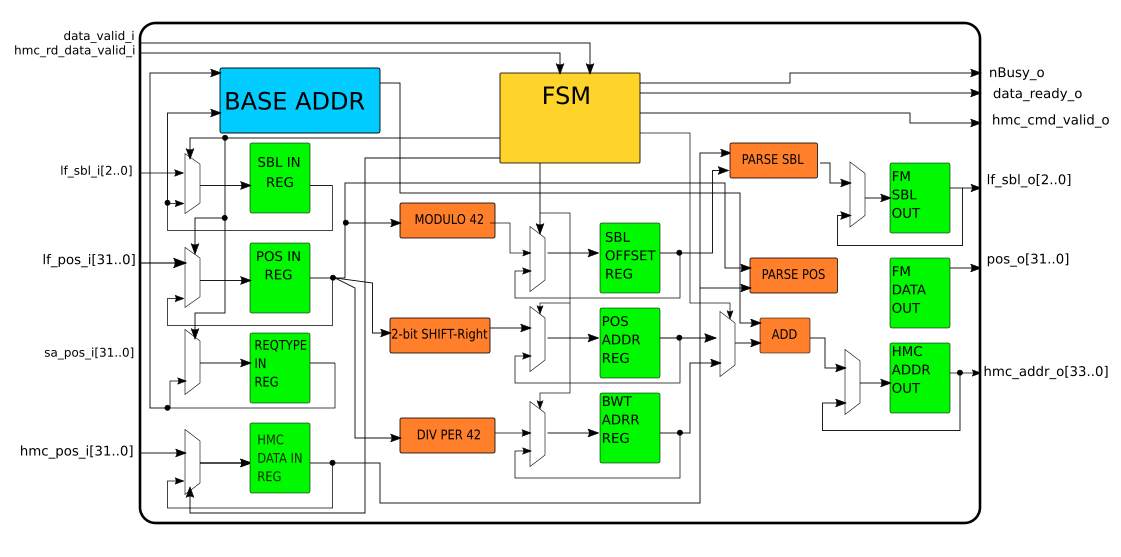
\includegraphics[scale = 0.45]{Figures/HMC_DIAG.png}
    \caption{HMC Interface Bloc Diagram}
    \label{fig:seqschema}
\end{figure}

\subsection{Timing Requirements}

Inherited from the project are the timing requirements for the system, set at 250MHz, meaning that in order to produce a bitmap for the FPGA that would be guaranteed to behave as written, there should be no paths longer than 4 ns for a signal between two storing elements or port. \\
Considering the global structure of the implemented system, most paths respect this constraint as most exchanged data are stored into local registers and most operations are simple.\\

Nonetheless, the HMC Interface bloc had a path that did not last under that 4 ns, this being due to a rather unpleasant but necessary operation done one the position provided by the FM-Index. In the case of a query for a symbol of the BWT, the actual address is calculated by dividing this position by the number of symbol contained in each row, meaning here the inconvenient number 42. This kind of division is synthesized into a series of numerous simpler operations (see Fig. \ref{fig:timing}) with by default no storage element in between, thus creating a long path upon which we have little to no control. \\

\begin{figure}[H]
    \centering
    \hspace*{-3mm}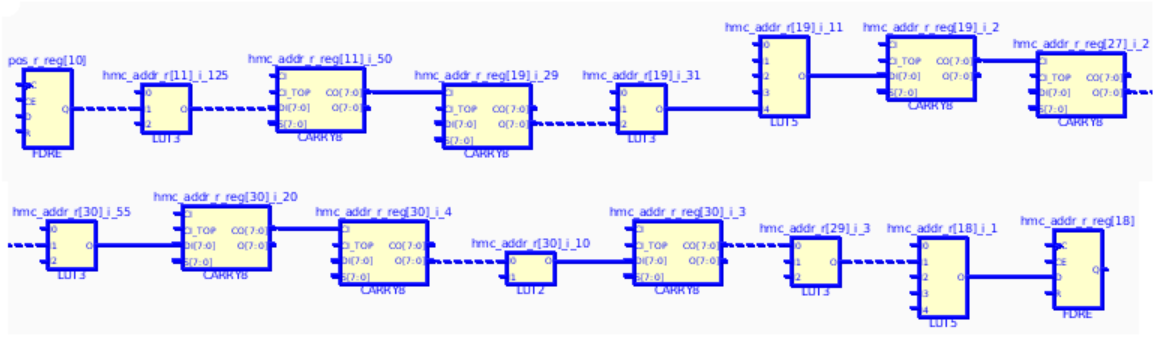
\includegraphics[scale = 0.4]{Figures/TIMING_RTL.png}
    \caption{RTL View of the hardware path generated}
    \label{fig:timing}
\end{figure}
TODO
After some digging [REFORMULER] it was enough to enable more control to the synthesizer on the timings and optimization of those kind of delays to reduce this time to just under 4 ns. 

Another solution would have been to simplify the problematic operation by encoding the BWT on 4 bits. This would have allowed 32 elements per memory row, and thus reducing the division to a simple 5-bit shift to the right in order to determine an element's row and its position in it. However, this would have increase the space needed to store 

\section{C++ Interface Implementation}

In order to be able to communicate with the board from a computer, it requires a interface enabling :
\begin{itemize}
    \item [-] writing directly into the main memory in order to store the references
    \item [-]writing parameters to addressed registers
    \item [-] sending the short reads via a stream
    \item [-] reading the results via a stream
\end{itemize}

Furthermore, it becomes necessary to generate references that would correspond to their usage in the hardware system, hence providing methods that would not only encode those references (BWT, sampled suffix-array and checkpoints) but also write those correctly into the HMC. Figure \ref{fig:memory} show the memory organization. Each row is 128-bit, little endian. \\

The first point will be further discussed in the section PicoFramework, as it highly relies on the framework provided by the board manufacturer.

\begin{minipage}[t]{0.4\textwidth}
\begin{figure}[H]
    \centering
    \hspace*{-10mm}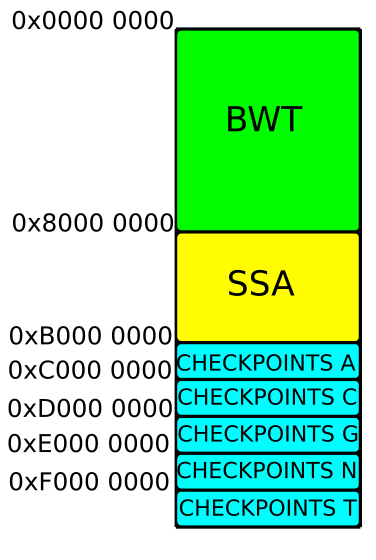
\includegraphics[scale = 0.4]{Figures/MEM_RPZ.png}
    \caption{Memory Organization}
    \label{fig:memory}
\end{figure}
\end{minipage}
\hfill
\begin{minipage}[t]{0.5\textwidth}

The biggest reference to store is the BWT with 3-bit values for each symbol, half of the memory is dedicated to it. \\
Then, the Sampled Suffix-Array with 32-bit values every 32 symbols (average 1 bit per symbol). \\
Finally the checkpoints, separated by symbol in order to simplify the address and the offset calculation, although it requires passing the requested symbol to the HMC Interface. For 5 symbols, it requires $5 * 32 / 128$ bits, so an average of 1.25 bit per symbol.\\
Hence, a total of 5.25 bits per symbol is necessary to store all the references, with a 4GiB memory, we can then process references up to $\approx 8.2*10^{8}$ symbols.
\end{minipage}

\vspace*{8mm}

\paragraph{BWT encoding}

In order to correctly encode the BWT, the number of element per row has to be taken into account. Considering there is no 128-bit integer type available to store data row per row, each one of those is split into two 64-bit unsigned integers. Considering the symbols are encoded on 3 bits, there is no way to fill each word with a round number of symbols. Hence, in order to keep the data coherent, for each row, the procedure is describer in Algorithm \ref{alg:bwt}.\\


\vspace*{5mm}


\begin{minipage}[t]{0.55\textwidth}
\begin{algorithm}[H]
	\SetAlgoLined
	\KwIn{BWT $T^{bwt}$ encoded as in section 2.3.1}
	\KwOut{vector of uint64\_t pairs}
	res = <>; \textit{\# Empty vector of uint64\_t pairs} \\
	temp = <>; \textit{\# Empty pair of uint64\_t} \\
	j = 0; \textit{\# Global Index}\\
	\For{each 42 symbols roW in $T^{bwt}$}{
		t = ""; \\
		\For{i = 0; i < 42; i++}{
		    t = to\_string(bwt[j]) + t;\\
		    j++;
		}
		temp[0] = str\_to\_integer(t[64..127], 2);
		temp[1] = str\_to\_integer(t[0..63], 2);
        res.append(temp);
	}
\caption{Encoding the BWT for Memory
}
\label{alg:bwt}
\end{algorithm}
\end{minipage}
 \hfill
\begin{minipage}[t]{0.3 \textwidth}
The string representation of each value is shown in the table below.
\vspace*{5mm}


\begin{tabular}{|c|c|}
\hline
Input    &  to\_string() result\\
\hline
 A    &  "010" \\
 C    &  "011" \\
 G    &  "100" \\
 N    &  "101" \\
 T    &  "110" \\
\hline
\end{tabular}
\vspace*{3mm}

The function \textit{str\_to\_integer} is given a string that it converts into an integer using the base provided as second argument to do the conversion. \\
\end{minipage}
\vspace*{5mm}


\textit{\underline{Note}} : If the number of symbols is not a multiple of 42, a last loop is done with the remainings values, padding the rest of the buffer row with '0's. \\



A string representation of each row must be done in order to correctly dispatch the bits between the two 64-bit words. Every string is constructed from the right to the left in order to place the first character where the least significant bits are (as it is interpreted by the conversion method - little endian). \\
Finally, the first element of each pair must represent the first 64 bits of the memory row, hence the indices [64..127] for the first 64-bit word, and [0..63] for the second that will be used for bits [63..0] and [127..64] respectively to write the memory row.

\paragraph{Sampled Suffix-Array and Checkpoints encoding}

All values from those references are stored in and used as 32-bit values. This round number allows 4 values per row and the order in which the written buffer is defined as follow :
\begin{enumerate}
    \item Fetch the next 4 values in an array \texttt{position[4]} of unsigned 32-bit integers with \texttt{position[0]} being the first fetched, etc.
    \item Convert each value into an hexadecimal representation
    \item Add this row to the final buffer
    \item Repeat from Step 1 until there is no value left
\end{enumerate}

\textit{\underline{Note}}: If the number of checkpoints or suffix-array sample is not a multiple of 4, this a last loop is done, padding the rest of the buffer row with '0's. \\

Both those encoding methods are passed a binary input file containing unsigned integer value for each position / symbol.

In the scope of this project, only a terminal interface will be implemented. It is used as follow :
\begin{enumerate}
    \item Launch the program providing either a bitmap or a project file corresponding to the system implemented for the FPGA
    \item Upon request, provide a FASTA file containing the reference genome
    \item Upon request, provide a FASTQ file containing the short reads to map onto the reference
    \item Upon notification, a text file should contain all the short reads reference followed by their position in the reference ('-1' if not found)
\end{enumerate}

The first step is further explained in the next section, as it fully takes advantage of the tools from the Pico Framework.


\subsection{Pico Framework}

This framework, provided by the board manufacturer, not only offers methods and tools to communicate with the board, but also a powerful way to simulate it and its execution. All the informations provided below are from the \textit{Pico User Guide}\cite{PICOO}.

\paragraph{Reaching the FPGA}
\begin{minted}{c}
PicoDrv *pico_ptr;
int FindPico(uint32_t model, PicoDrv **drvpp);
int RunBitFile(const char *bitFilePath, PicoDrv **drvpp);
\end{minted}

In order to be able to detect and link the FPGA, it is first necessary to declare a \texttt{PicoDrv} instance that will then provide all the methods in the next paragraphs. \\
The pointer is instantiated using the \texttt{FinPico} method, providing it also an index corresponding to the FPGA model (\texttt{0x510} in this project).\\
Then, the method \texttt{RunBitFile}, provided the aforementioned pointer and the path to a bitStream file, is used to program the FPGA with a compiled hardware system. \\
Note that this last method can also be provided a project descriptor (Vivado or Quartus) in order to launch a simulation. This aspect will be further discussed in Section 4.4.


\paragraph{Writing to the Memory} \\
\begin{minted}{c}
int WriteRam(uint64_t addr, const void * buf, int size, int memID);
\end{minted}
The address provided must be 16-Byte align, along with \texttt{buf} containing the data to write. Further more, \texttt{size} represents the number of bytes to write, it must also be a multiple of 16. Finally, \texttt{memID} indicates the ID of the memory to which we want to write, in this project, the required value is 0. \\

The first word of the buffer will be placed at the first byte of the memory row, hence the buffer is big-endian word-wise. For each word however, the value is read as a little endian.

\paragraph{Writing to and Ready from the Stream}
\begin{minted}{c}
int createStream(int streamID);
int ReadStream(int streamHandle, void * buf, size_t count);
int WriteStream(int streamHandle, const void * buf, size_t count);
\end{minted}
The first method is used to instanciate a handler for the stream that will then be needed for the two other methods. \\

The two following methods are used to respectively write to and read from the PCI stream between the computer and the FPGA. Considering the bus is a stream in this case, there are no addresses to provide but the \texttt{count} value is still required to be a multiple of the stream width in bytes, in this case, 16.

\section{Co-Simulation}

In order to facilitate the debug process, the Pico Framework offers a way to simulate the board instead of loading it to test the developped application. Doing so is rather simple : it is enough to provide the program a project file (e.g. \texttt{.fwproj} for Vivado, \texttt{.qpf} for Quartus).\\

This allowed us to thoroughly test the implemented system with a simulation very close to the reality. Despite being hard to read, the simulation provides all the desired signals inside the system, thus allowing for a deep inspection of its behavior.

\subsection{Constated Issues}

As a result to those simulations, several issues have been noted that did not occur in the previously mentioned testbenches :
\begin{itemize}
    \item [-] The endianness of the memory must be dealt with in order for the data to be coherent. Unexpectedly, it was a major issue during the test phase and on several occasions was the reason the system was failing.
    \item [-] The HMC memory bus' contain all '0' when not used. The requested data is only available for 1 clock period and thus, has to be latched immediately.
    \item [-] The PicoBus, from which the parameters registers are written, not only is used by the framework and thus, the address decoder must be restricted to a certain address range. But it also has a clock very much slower than the internal system clock. Hence, it is necessary deal with this by re-synchronizing the received data.
\end{itemize}

\section{On-Board Testing}
TODO
\section{Validation}

In order to validate the system, the reference used in Chapter 3 has been used and some mock short reads extracted from it are used as input, this time, as is (meaning here as a text and not already processed data). \\

The results were quite satisfying, as all the bugs had been detected during the simulation process. \\

Despite being a little over the restriction (less than 0.1 ns) for a couple a paths, the system seems to behave correctly in normal conditions (low temperature and low demand).
